\documentclass[conference]{IEEEtran}
\usepackage{hyperref}
\usepackage{graphics} % Required for the inclusion of images
\usepackage{graphicx} % Required for the inclusion of images
\usepackage{caption}
\usepackage{amssymb}
\usepackage{amsmath}
\usepackage{subfigure}
\usepackage{pifont}
\usepackage{tikz}
\usepackage{pgfplots}
\usepackage{textcomp}
\usepackage{standalone}
\usepackage{import}
\usepackage{lipsum}
\usetikzlibrary{patterns}
\newcommand{\blue}[1]{\textcolor{blue}{#1}}
\newcommand{\red}[1]{\textcolor{red}{#1}}
\title{\LaTeX\, Gallery}

\author{
    \IEEEauthorblockN{Junyan Su}
    \IEEEauthorblockA{junyan.su@my.cityu.edu.hk}
}

\begin{document}
\maketitle

\begin{abstract}
    This is a small gallery of latex examples. I found some good figures/tables in the literature and reproduce them with latex. Every example corresponds to a standalone tex file in the folder submodules. A github repository is also available\footnote{\url{https://github.com/sujunyan/tex-gallery}}.
\end{abstract}


\begin{IEEEkeywords}
    \LaTeX , Figure, Table
\end{IEEEkeywords}

\section{Introduction}
% figure 2a/2b ----------------------
\lipsum[1]
\begin{figure}[tb]
    \begin{center}
        \subfigure[A subcaption]{
            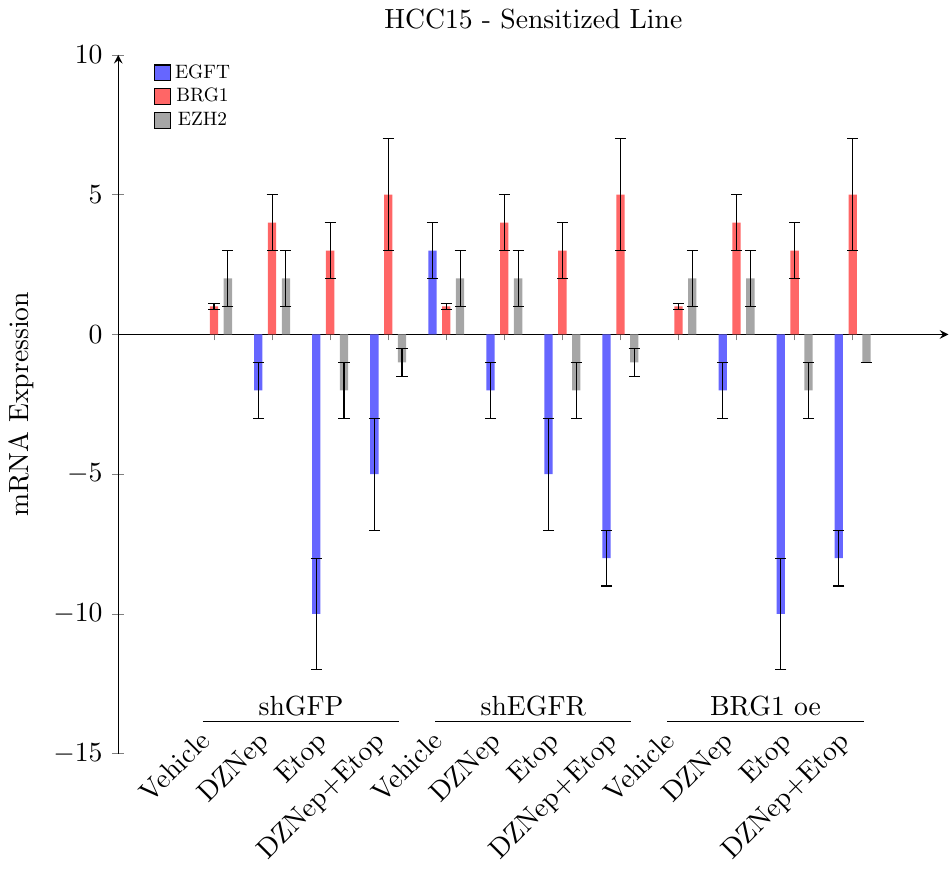
\includegraphics[width=\linewidth]{submodules/2a/2a.pdf}
        }
        \subfigure[A subcaption]{
            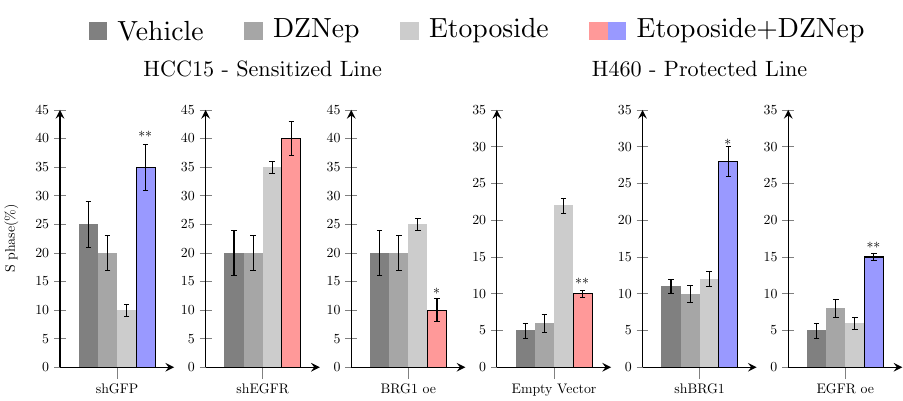
\includegraphics[width=\linewidth]{submodules/2b/2b.pdf}
        }
        %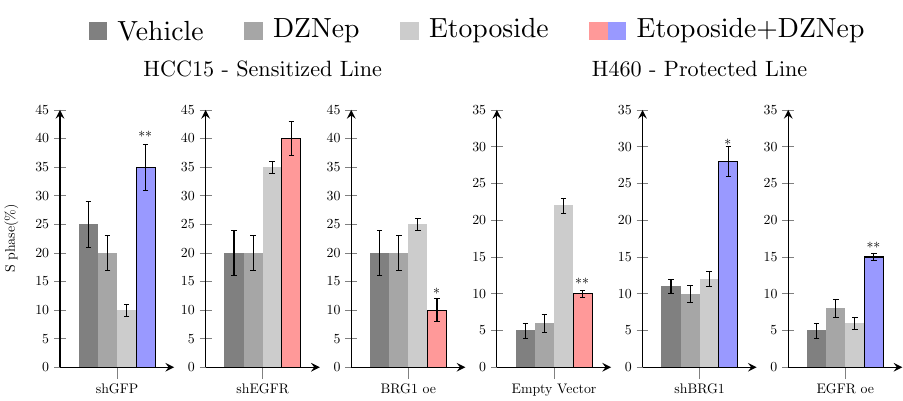
\includegraphics[width=\linewidth]{submodules/2b/2b.pdf}
    \end{center} 
    \caption{Two of the sub-figures from Extended Data Figure 8 in~\cite{2}.}
\end{figure}

\lipsum[1]
\begin{figure*}[htb]
    \begin{center}
        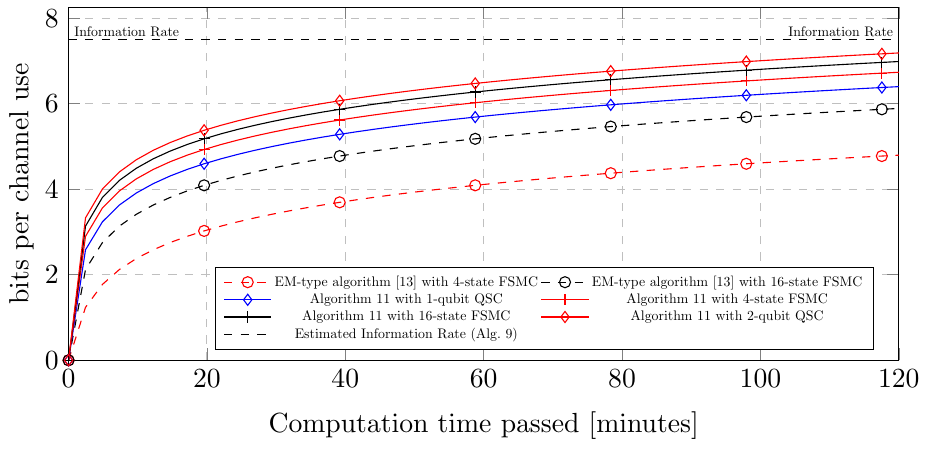
\includegraphics[width=\linewidth]{submodules/1/1.pdf}
    \end{center} 
    \caption{This is fig.11 from~\cite{1}}
\end{figure*}

% figure 3a/3b -----------------------------
\lipsum
\begin{figure*}[htb]
    \begin{center}
        \subfigure[A subcaption]{
            %\includestandalone[width=.48\linewidth]{submodules/3a/3a}
            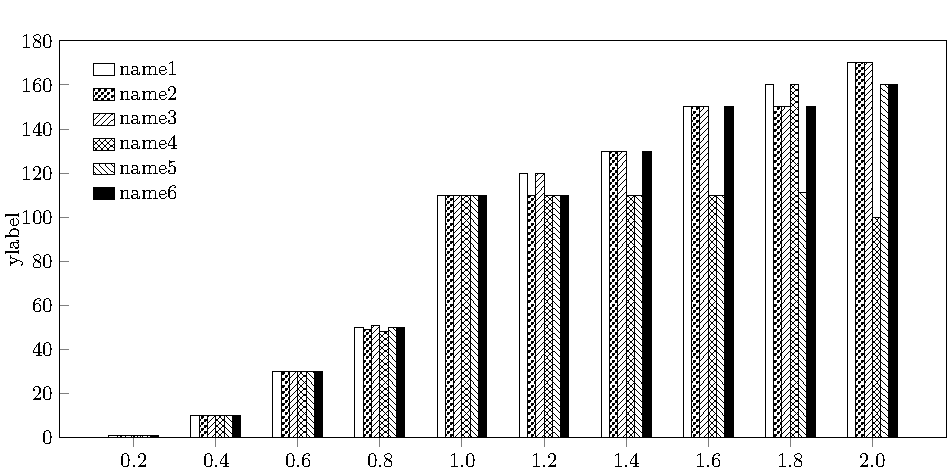
\includegraphics[width=0.48\linewidth]{submodules/3a/3a.pdf}
        }
        \subfigure[A subcaption]{
            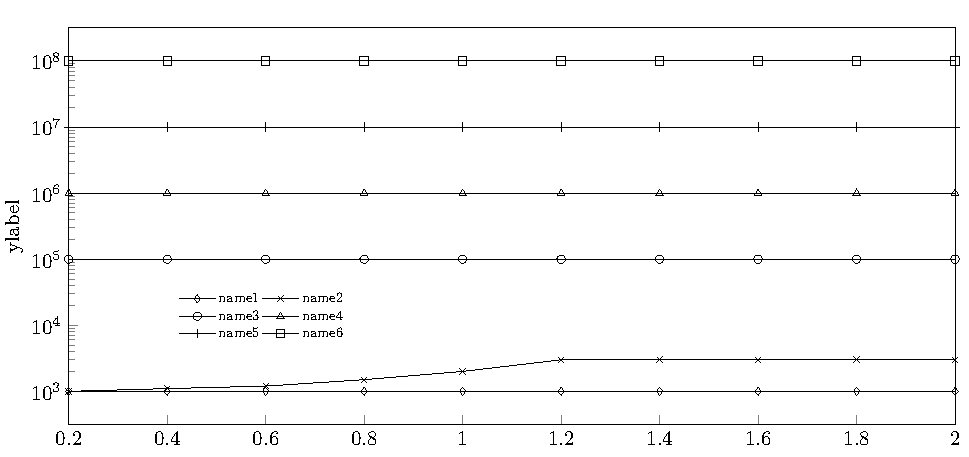
\includegraphics[width=0.48\linewidth]{submodules/3b/3b.pdf}
            %\includestandalone[width=.48\linewidth]{submodules/3b/3b}
        }
    \end{center} 
    \caption{(A figure across two columns)}
\end{figure*}

% usage \includeSubmodule{name}{additional caption}{*?}
\newcommand{\includeSubmodule}[3]{
    \begin{figure#3}[!htb]
        \begin{center}
            \includegraphics[width=\linewidth]{submodules/#1/#1.pdf}
        \end{center} 
        \caption{#2}
    \end{figure#3}
}

\lipsum[1]
\includeSubmodule{4}{pcode example}{}
\lipsum[1]
\includeSubmodule{6}{table example 02}{*}
\lipsum[1]

\newcommand{\xmark}{\ding{55}}%package pifont
\begin{table}[h]
  \begin{tabular}{|c|c|c|c|}
    \hline
    Paper & Route Planning & Speed Planning & Hard Deadline \\  \hline
    [37] & \checkmark & \xmark & \xmark \\ \hline
    [16] & \xmark & \checkmark & \xmark \\ \hline
    [17] & \xmark & \checkmark &  \checkmark \\ \hline
    This work & \checkmark&\checkmark & \checkmark\\ \hline
  \end{tabular}
  \caption{Table~II from~\cite{deng2017energy}}
\end{table}
\lipsum
\includeSubmodule{5}{table example 01}{*}
\lipsum

\bibliographystyle{unsrt}
\bibliography{ref}
\end{document}